% Options for packages loaded elsewhere
% Options for packages loaded elsewhere
\PassOptionsToPackage{unicode}{hyperref}
\PassOptionsToPackage{hyphens}{url}
%
\documentclass[
  ignorenonframetext,
  aspectratio=43,
]{beamer}
\newif\ifbibliography
\usepackage{pgfpages}
\setbeamertemplate{caption}[numbered]
\setbeamertemplate{caption label separator}{: }
\setbeamercolor{caption name}{fg=normal text.fg}
\beamertemplatenavigationsymbolsempty
% remove section numbering
\setbeamertemplate{part page}{
  \centering
  \begin{beamercolorbox}[sep=16pt,center]{part title}
    \usebeamerfont{part title}\insertpart\par
  \end{beamercolorbox}
}
\setbeamertemplate{section page}{
  \centering
  \begin{beamercolorbox}[sep=12pt,center]{section title}
    \usebeamerfont{section title}\insertsection\par
  \end{beamercolorbox}
}
\setbeamertemplate{subsection page}{
  \centering
  \begin{beamercolorbox}[sep=8pt,center]{subsection title}
    \usebeamerfont{subsection title}\insertsubsection\par
  \end{beamercolorbox}
}
% Prevent slide breaks in the middle of a paragraph
\widowpenalties 1 10000
\raggedbottom
\AtBeginPart{
  \frame{\partpage}
}
\AtBeginSection{
  \ifbibliography
  \else
    \frame{\sectionpage}
  \fi
}
\AtBeginSubsection{
  \frame{\subsectionpage}
}
\usepackage{iftex}
\ifPDFTeX
  \usepackage[T1]{fontenc}
  \usepackage[utf8]{inputenc}
  \usepackage{textcomp} % provide euro and other symbols
\else % if luatex or xetex
  \usepackage{unicode-math} % this also loads fontspec
  \defaultfontfeatures{Scale=MatchLowercase}
  \defaultfontfeatures[\rmfamily]{Ligatures=TeX,Scale=1}
\fi
\usepackage{lmodern}

\usetheme[]{Madrid}
\usecolortheme[]{default}
\usefonttheme[]{structurebold}
\ifPDFTeX\else
  % xetex/luatex font selection
\fi
% Use upquote if available, for straight quotes in verbatim environments
\IfFileExists{upquote.sty}{\usepackage{upquote}}{}
\IfFileExists{microtype.sty}{% use microtype if available
  \usepackage[]{microtype}
  \UseMicrotypeSet[protrusion]{basicmath} % disable protrusion for tt fonts
}{}
\makeatletter
\@ifundefined{KOMAClassName}{% if non-KOMA class
  \IfFileExists{parskip.sty}{%
    \usepackage{parskip}
  }{% else
    \setlength{\parindent}{0pt}
    \setlength{\parskip}{6pt plus 2pt minus 1pt}}
}{% if KOMA class
  \KOMAoptions{parskip=half}}
\makeatother

\usepackage{color}
\usepackage{fancyvrb}
\newcommand{\VerbBar}{|}
\newcommand{\VERB}{\Verb[commandchars=\\\{\}]}
\DefineVerbatimEnvironment{Highlighting}{Verbatim}{commandchars=\\\{\}}
% Add ',fontsize=\small' for more characters per line
\usepackage{framed}
\definecolor{shadecolor}{RGB}{241,243,245}
\newenvironment{Shaded}{\begin{snugshade}}{\end{snugshade}}
\newcommand{\AlertTok}[1]{\textcolor[rgb]{0.68,0.00,0.00}{#1}}
\newcommand{\AnnotationTok}[1]{\textcolor[rgb]{0.37,0.37,0.37}{#1}}
\newcommand{\AttributeTok}[1]{\textcolor[rgb]{0.40,0.45,0.13}{#1}}
\newcommand{\BaseNTok}[1]{\textcolor[rgb]{0.68,0.00,0.00}{#1}}
\newcommand{\BuiltInTok}[1]{\textcolor[rgb]{0.00,0.23,0.31}{#1}}
\newcommand{\CharTok}[1]{\textcolor[rgb]{0.13,0.47,0.30}{#1}}
\newcommand{\CommentTok}[1]{\textcolor[rgb]{0.37,0.37,0.37}{#1}}
\newcommand{\CommentVarTok}[1]{\textcolor[rgb]{0.37,0.37,0.37}{\textit{#1}}}
\newcommand{\ConstantTok}[1]{\textcolor[rgb]{0.56,0.35,0.01}{#1}}
\newcommand{\ControlFlowTok}[1]{\textcolor[rgb]{0.00,0.23,0.31}{\textbf{#1}}}
\newcommand{\DataTypeTok}[1]{\textcolor[rgb]{0.68,0.00,0.00}{#1}}
\newcommand{\DecValTok}[1]{\textcolor[rgb]{0.68,0.00,0.00}{#1}}
\newcommand{\DocumentationTok}[1]{\textcolor[rgb]{0.37,0.37,0.37}{\textit{#1}}}
\newcommand{\ErrorTok}[1]{\textcolor[rgb]{0.68,0.00,0.00}{#1}}
\newcommand{\ExtensionTok}[1]{\textcolor[rgb]{0.00,0.23,0.31}{#1}}
\newcommand{\FloatTok}[1]{\textcolor[rgb]{0.68,0.00,0.00}{#1}}
\newcommand{\FunctionTok}[1]{\textcolor[rgb]{0.28,0.35,0.67}{#1}}
\newcommand{\ImportTok}[1]{\textcolor[rgb]{0.00,0.46,0.62}{#1}}
\newcommand{\InformationTok}[1]{\textcolor[rgb]{0.37,0.37,0.37}{#1}}
\newcommand{\KeywordTok}[1]{\textcolor[rgb]{0.00,0.23,0.31}{\textbf{#1}}}
\newcommand{\NormalTok}[1]{\textcolor[rgb]{0.00,0.23,0.31}{#1}}
\newcommand{\OperatorTok}[1]{\textcolor[rgb]{0.37,0.37,0.37}{#1}}
\newcommand{\OtherTok}[1]{\textcolor[rgb]{0.00,0.23,0.31}{#1}}
\newcommand{\PreprocessorTok}[1]{\textcolor[rgb]{0.68,0.00,0.00}{#1}}
\newcommand{\RegionMarkerTok}[1]{\textcolor[rgb]{0.00,0.23,0.31}{#1}}
\newcommand{\SpecialCharTok}[1]{\textcolor[rgb]{0.37,0.37,0.37}{#1}}
\newcommand{\SpecialStringTok}[1]{\textcolor[rgb]{0.13,0.47,0.30}{#1}}
\newcommand{\StringTok}[1]{\textcolor[rgb]{0.13,0.47,0.30}{#1}}
\newcommand{\VariableTok}[1]{\textcolor[rgb]{0.07,0.07,0.07}{#1}}
\newcommand{\VerbatimStringTok}[1]{\textcolor[rgb]{0.13,0.47,0.30}{#1}}
\newcommand{\WarningTok}[1]{\textcolor[rgb]{0.37,0.37,0.37}{\textit{#1}}}

\usepackage{longtable,booktabs,array}
\usepackage{calc} % for calculating minipage widths
\usepackage{caption}
% Make caption package work with longtable
\makeatletter
\def\fnum@table{\tablename~\thetable}
\makeatother
\usepackage{graphicx}
\makeatletter
\newsavebox\pandoc@box
\newcommand*\pandocbounded[1]{% scales image to fit in text height/width
  \sbox\pandoc@box{#1}%
  \Gscale@div\@tempa{\textheight}{\dimexpr\ht\pandoc@box+\dp\pandoc@box\relax}%
  \Gscale@div\@tempb{\linewidth}{\wd\pandoc@box}%
  \ifdim\@tempb\p@<\@tempa\p@\let\@tempa\@tempb\fi% select the smaller of both
  \ifdim\@tempa\p@<\p@\scalebox{\@tempa}{\usebox\pandoc@box}%
  \else\usebox{\pandoc@box}%
  \fi%
}
% Set default figure placement to htbp
\def\fps@figure{htbp}
\makeatother





\setlength{\emergencystretch}{3em} % prevent overfull lines

\providecommand{\tightlist}{%
  \setlength{\itemsep}{0pt}\setlength{\parskip}{0pt}}



 


\usepackage{booktabs}
\definecolor{darkblue}{RGB}{10, 45, 90}
\setbeamercolor{title page background}{fg=white, bg=darkblue}
\setbeamercolor{palette primary}{bg=darkblue, fg=white}
\setbeamercolor{palette secondary}{bg=darkblue, fg=white}
\setbeamercolor{palette tertiary}{bg=darkblue, fg=white}
\setbeamercolor{palette quaternary}{bg=darkblue, fg=white}
\setbeamercolor{frametitle}{bg=darkblue, fg=white}
\setbeamercolor{title separator}{fg=darkblue}
\setbeamercolor{progress bar}{fg=darkblue}
\setbeamerfont{title}{size=\LARGE}
\setbeamerfont{subtitle}{size=\large}
\setbeamertemplate{footline}{}
\setbeamertemplate{navigation symbols}{}
\setbeamercolor{block title}{bg=darkblue, fg=white}
\setbeamercolor{block body}{bg=darkblue!10, fg=black}
\setbeamerfont{title}{size=\LARGE}
\setbeamerfont{subtitle}{size=\large}
\setbeamertemplate{footline}{}
\setbeamertemplate{navigation symbols}{}
\makeatletter
\@ifpackageloaded{caption}{}{\usepackage{caption}}
\AtBeginDocument{%
\ifdefined\contentsname
  \renewcommand*\contentsname{Table of contents}
\else
  \newcommand\contentsname{Table of contents}
\fi
\ifdefined\listfigurename
  \renewcommand*\listfigurename{List of Figures}
\else
  \newcommand\listfigurename{List of Figures}
\fi
\ifdefined\listtablename
  \renewcommand*\listtablename{List of Tables}
\else
  \newcommand\listtablename{List of Tables}
\fi
\ifdefined\figurename
  \renewcommand*\figurename{Figure}
\else
  \newcommand\figurename{Figure}
\fi
\ifdefined\tablename
  \renewcommand*\tablename{Table}
\else
  \newcommand\tablename{Table}
\fi
}
\@ifpackageloaded{float}{}{\usepackage{float}}
\floatstyle{ruled}
\@ifundefined{c@chapter}{\newfloat{codelisting}{h}{lop}}{\newfloat{codelisting}{h}{lop}[chapter]}
\floatname{codelisting}{Listing}
\newcommand*\listoflistings{\listof{codelisting}{List of Listings}}
\makeatother
\makeatletter
\makeatother
\makeatletter
\@ifpackageloaded{caption}{}{\usepackage{caption}}
\@ifpackageloaded{subcaption}{}{\usepackage{subcaption}}
\makeatother

\usepackage{bookmark}
\IfFileExists{xurl.sty}{\usepackage{xurl}}{} % add URL line breaks if available
\urlstyle{same}
\hypersetup{
  pdftitle={Human Development Index (HDI) in Sub-Saharan Africa},
  pdfauthor={Gruppo F: Bondi, Dal Ben, Michetti, Proietti, Veronese},
  hidelinks,
  pdfcreator={LaTeX via pandoc}}


\title{Human Development Index (HDI) in Sub-Saharan Africa}
\subtitle{Un'analisi comparativa: Nigeria, Ghana, Senegal, Sudafrica}
\author{Gruppo F: Bondi, Dal Ben, Michetti, Proietti, Veronese}
\date{2026-05-14}

\begin{document}
\frame{\titlepage}


\begin{frame}{Dove eravamo rimasti - HDI e sviluppo umano in Africa
Sub-Sahariana}
\phantomsection\label{dove-eravamo-rimasti---hdi-e-sviluppo-umano-in-africa-sub-sahariana}
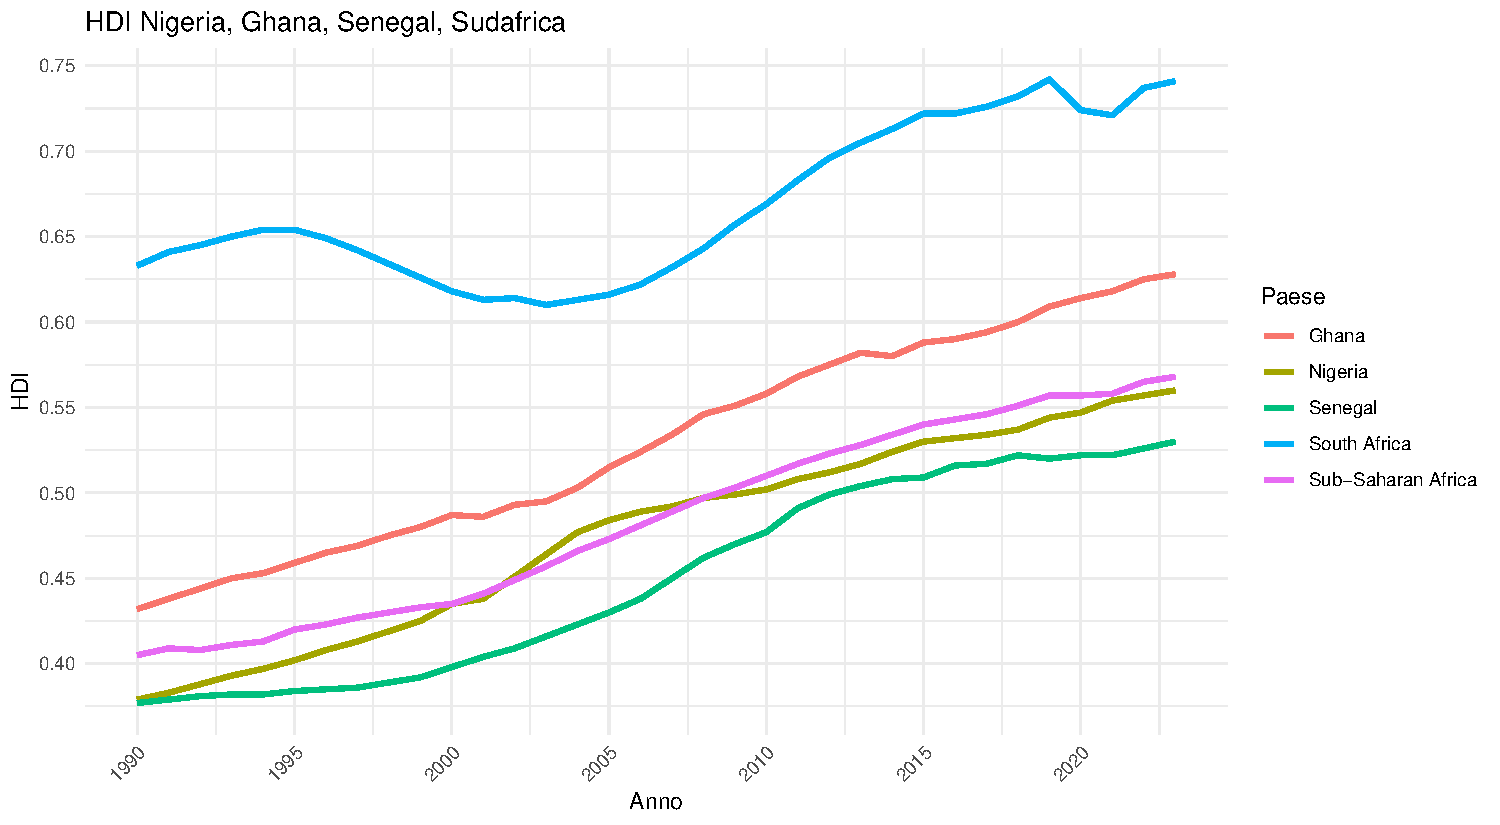
\includegraphics[width=1\linewidth,height=\textheight,keepaspectratio]{pres.final_files/figure-beamer/plot-hdi-country1-1.pdf}
\end{frame}

\begin{frame}{Analisi precedenti - GDP per capita (current US\$) nei 4
paesi}
\phantomsection\label{analisi-precedenti---gdp-per-capita-current-us-nei-4-paesi}
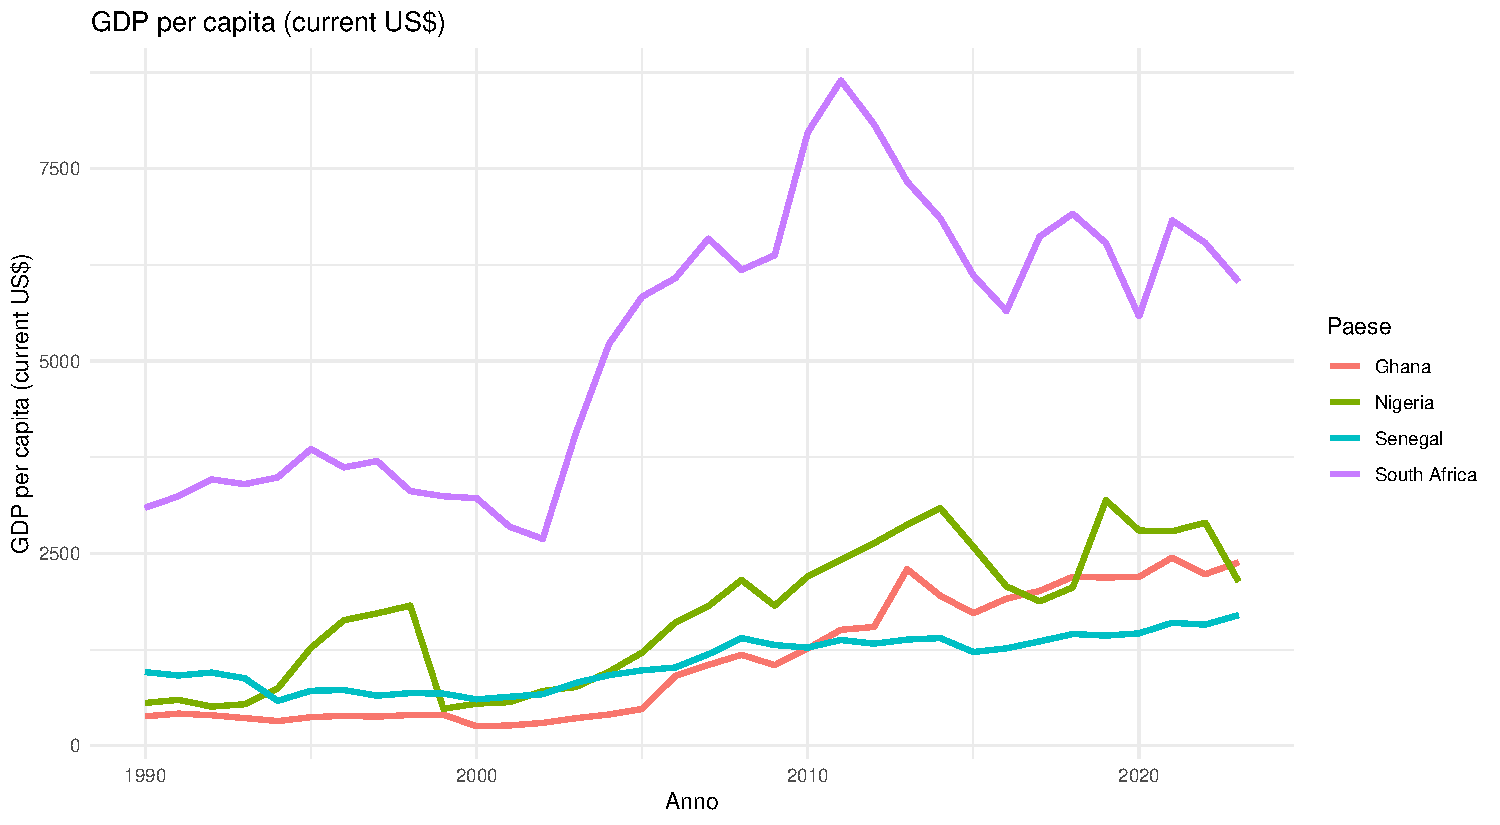
\includegraphics[width=1\linewidth,height=\textheight,keepaspectratio]{pres.final_files/figure-beamer/plot-gdp-country-1.pdf}
\end{frame}

\begin{frame}{Obiettivi dell'analisi}
\phantomsection\label{obiettivi-dellanalisi}
\begin{columns}[T]
\begin{column}{0.45\linewidth}
\begin{block}{Fase 1: HDI globale}
Confrontare l'andamento dell'\textbf{Indice di Sviluppo Umano (HDI)} nell'Africa Sub-Sahariana rispetto al resto del mondo (1990--2023)
\end{block}
\end{column}

\vspace{0.5cm}

\begin{column}{0.45\linewidth}
\begin{block}{Fase 2: Confronto tra paesi}
Analizzare le differenze tra \textbf{Nigeria, Ghana, Senegal e Sudafrica} su indicatori chiave: PIL, fertilità, acqua, elettricità, mortalità
\end{block}
\end{column}
\end{columns}
\end{frame}

\begin{frame}{Domande di ricerca}
\phantomsection\label{domande-di-ricerca}
\begin{columns}[T]
\begin{column}{0.45\linewidth}
\begin{block}{Domanda 1: Determinanti dell'HDI}
La crescita economica si traduce in miglioramenti dell'HDI? Quali sono i determinanti più influenti?
\end{block}
\end{column}

\vspace{0.5cm}

\begin{column}{0.45\linewidth}
\begin{block}{Domanda 2: Shock globali}
Qual è stato l'impatto delle crisi globali (2008, COVID-19) sull'HDI nei paesi analizzati? Esistono differenze significative nella resilienza tra i paesi?
\end{block}
\end{column}
\end{columns}

\vspace{0.5em}

\textit{Dati: UNDP Human Development Report, World Bank Open Data}
\end{frame}

\begin{frame}{Studio preliminare: Matrice di Correlazione}
\phantomsection\label{studio-preliminare-matrice-di-correlazione}
\begin{columns}[T]
\begin{column}{0.5\linewidth}
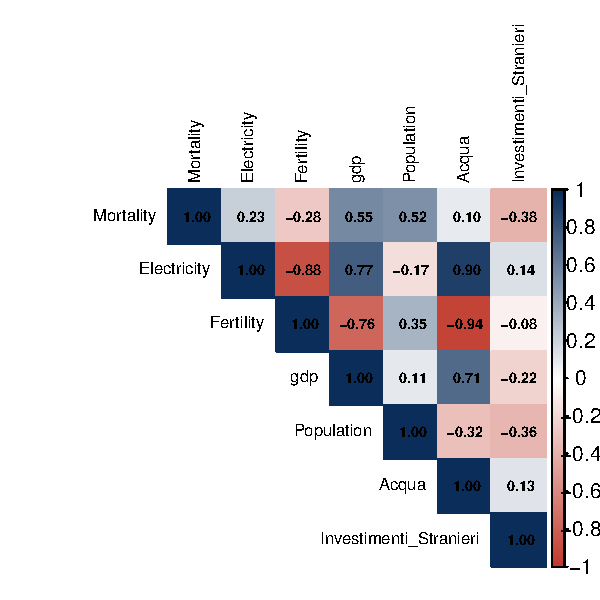
\includegraphics[width=1\linewidth,height=\textheight,keepaspectratio]{pres.final_files/figure-beamer/plot-corrplot-slide-1.pdf}
\end{column}

\begin{column}{0.5\linewidth}
\small

\textbf{Osservazioni chiave:}

\begin{itemize}
  \item Forte correlazione tra fecondità, elettricità e accesso all'acqua.
  \item \textbf{GDP}: correlato con elettricità (0.76) e acqua (0.69), ma meno con le altre variabili.
  \item \textbf{FDI}: correlazioni deboli con tutte le variabili → regressore relativamente indipendente.
\end{itemize}
\end{column}
\end{columns}
\end{frame}

\begin{frame}{Modelli econometrici: Strategia di stima}
\phantomsection\label{modelli-econometrici-strategia-di-stima}
\begin{block}{Modello 1 - Effetti fissi con interazioni PLM}
Controlla per eterogeneità non osservata stabile nel tempo
\end{block}

\vspace{0.4em}

\begin{itemize}
  \item \textbf{Interazioni variabile $\times$ paese} — slope eterogenei: ogni paese reagisce diversamente ai regressori
  \item \textbf{Errori standard robusti (HC1)} — correggono per eteroschedasticità
  \item Variabili incluse: mortalità, elettricità, fertilità, $\log(\text{GDP})$, accesso all'acqua, FDI
\end{itemize}

\vspace{0.4em}

\begin{block}{Modello 2}
Aggiunta di dummy crisi: \textit{crisi finanziaria 2008--09} e \textit{COVID-19 2020--21}
\end{block}
\end{frame}

\begin{frame}{Modello 1 --- Effetti fissi con interazioni}
\phantomsection\label{modello-1-effetti-fissi-con-interazioni}
Il modello \textit{within} stima l'impatto dei regressori sull'HDI: \[
\text{HDI}_{it} = \alpha_i + \beta_1 \text{Mort}_{it} + \beta_2 \text{Ele}_{it} + \beta_3 \text{Fert}_{it} + \beta_4 \log(\text{GDP})_{it} + \beta_5 \text{Wat}_{it} + \epsilon_{it}
\]

\begin{itemize}
  \item \textbf{Variabile Dipendente ($HDI_{it}$)}: Rappresenta l'Indice di Sviluppo Umano osservato per il paese $i$ nell'anno $t$.
  \item $\alpha_i$: Cattura le caratteristiche strutturali di ogni paese che non variano nel tempo (cultura, posizione geografica, istituzioni storiche).
  \item \textbf{Vettore dei Regressori $\beta_j$}: Variabili demografiche (\textit{Mortalità, Fertilità}) e infrastrutturali (\textit{Elettricità, Acqua, PIL}) per individuare l'effetto delle variazioni temporali di ogni regressore sull'HDI all'interno di ciascun paese.
\end{itemize}
\end{frame}

\begin{frame}{Modello 1 --- Effetti fissi con interazioni PLM}
\phantomsection\label{modello-1-effetti-fissi-con-interazioni-plm}
\begin{itemize}
  \item \textbf{Logaritmo del PIL ($\log(GDP)$)}: La trasformazione logaritmica permette di interpretare il coefficiente $\beta_4$ come l'elasticità dell'HDI rispetto alla crescita economica.
  \item \textbf{Termine di Errore ($\epsilon_{it}$)}: Cattura le fluttuazioni stocastiche e le componenti non osservate tempo-varianti.
\end{itemize}

\vspace{0.5cm}

\begin{block}{Obiettivo della Stima}
Stimare la significatività statistica e l'intensità di ogni canale di sviluppo a parità degli altri fattori.
\end{block}
\end{frame}

\begin{frame}{Scelta Metodologica: Lo stimatore Fixed Effects (Within)}
\phantomsection\label{scelta-metodologica-lo-stimatore-fixed-effects-within}
\begin{itemize}
  \item \textbf{Differenze strutturali tra paesi} (es. clima, risorse naturali) possono influenzare l'HDI ma non variano nel tempo
  \item \textbf{Eterogeneità non osservata} $\rightarrow$ ogni paese ha un suo "punto di partenza" dell'HDI
  \item \textbf{Intercetta $\alpha_i$ specifica per ogni paese}: cattura le differenze strutturali fisse che influenzano l'HDI
\end{itemize}
\end{frame}

\begin{frame}{Scelta Metodologica: Lo stimatore Fixed Effects (Within)}
\phantomsection\label{scelta-metodologica-lo-stimatore-fixed-effects-within-1}
\begin{itemize}
  \item \textbf{Analisi delle variazioni Within}: I coefficienti riflettono l'impatto delle variazioni temporali interne a ciascun paese, isolando l'effetto dinamico delle variabili indipendenti
  \item \textbf{Interpretazione interazioni}: i coefficienti stimati delle \textbf{interazioni} riflettono solo l'effetto delle variazioni temporali all'interno di ogni paese
  \item \textbf{Riduzione \textit{omitted variable bias}} $\rightarrow$  stima più accurata del nesso tra PIL, demografia e sviluppo umano (HDI).
\end{itemize}
\end{frame}

\begin{frame}[fragile]{Test di diagnostica - Eteroschedasticità}
\phantomsection\label{test-di-diagnostica---eteroschedasticituxe0}
\begin{Shaded}
\begin{Highlighting}[]
\FunctionTok{library}\NormalTok{(lmtest)}
\FunctionTok{bptest}\NormalTok{(model)}
\end{Highlighting}
\end{Shaded}

\begin{verbatim}

    studentized Breusch-Pagan test

data:  model
BP = 46.767, df = 27, p-value = 0.01051
\end{verbatim}

Il test di Breusch-Pagan evidenzia la presenza di eteroschedasticità
(p-value = 0.01051 \textless{} 0.05). Si è scelto di utilizzare errori
standard robusti HC1 per correggere questo problema.
\end{frame}

\begin{frame}{Coefficienti --- Acqua ed Elettricità}
\phantomsection\label{coefficienti-acqua-ed-elettricituxe0}
\begin{tabular}{lrrl}
\toprule
  & Coefficiente & P-value & Significativo\\
\midrule
Acqua & 0.0077 & 0.0000 & ***\\
Nigeria:Acqua & -0.0051 & 0.0004 & ***\\
Senegal:Acqua & -0.0013 & 0.3706 & \\
South Africa:Acqua & -0.0012 & 0.4746 & \\
Electricity & -0.0003 & 0.1559 & \\
\addlinespace
Nigeria:Electricity & 0.0004 & 0.3340 & \\
Senegal:Electricity & 0.0003 & 0.3698 & \\
South Africa:Electricity & 0.0017 & 0.0001 & ***\\
\bottomrule
\end{tabular}
\end{frame}

\begin{frame}{Coefficienti --- Investimenti Stranieri e log(GDP)}
\phantomsection\label{coefficienti-investimenti-stranieri-e-loggdp}
\resizebox{\textwidth}{!}{
\begin{tabular}{lrrl}
\toprule
  & Coefficiente & P-value & Significativo\\
\midrule
Investimenti\_Stranieri & 0.0013 & 0.0035 & **\\
Nigeria:Investimenti\_Stranieri & 0.0007 & 0.7000 & \\
Senegal:Investimenti\_Stranieri & -0.0027 & 0.0000 & ***\\
South Africa:Investimenti\_Stranieri & -0.0003 & 0.5640 & \\
log(gdp) & 0.0089 & 0.0253 & *\\
\addlinespace
Nigeria:log(gdp) & 0.0013 & 0.8353 & \\
Senegal:log(gdp) & 0.0030 & 0.6745 & \\
South Africa:log(gdp) & 0.0043 & 0.5399 & \\
\bottomrule
\end{tabular}

}
\end{frame}

\begin{frame}{Coefficienti --- Fertilità e Mortalità}
\phantomsection\label{coefficienti-fertilituxe0-e-mortalituxe0}
\begin{tabular}{lrrl}
\toprule
  & Coefficiente & P-value & Significativo\\
\midrule
Fertility & 0.0272 & 0.0374 & *\\
Nigeria:Fertility & -0.0236 & 0.1158 & \\
Senegal:Fertility & 0.0053 & 0.7094 & \\
South Africa:Fertility & -0.0450 & 0.0176 & *\\
Mortality & 0.0000 & 0.8772 & \\
\addlinespace
Mortality:Nigeria & -0.0003 & 0.3130 & \\
Mortality:Senegal & -0.0002 & 0.3860 & \\
Mortality:South Africa & -0.0004 & 0.0600 & .\\
\bottomrule
\end{tabular}
\end{frame}

\begin{frame}{Relazione tra reddito e sviluppo umano per paese}
\phantomsection\label{relazione-tra-reddito-e-sviluppo-umano-per-paese}
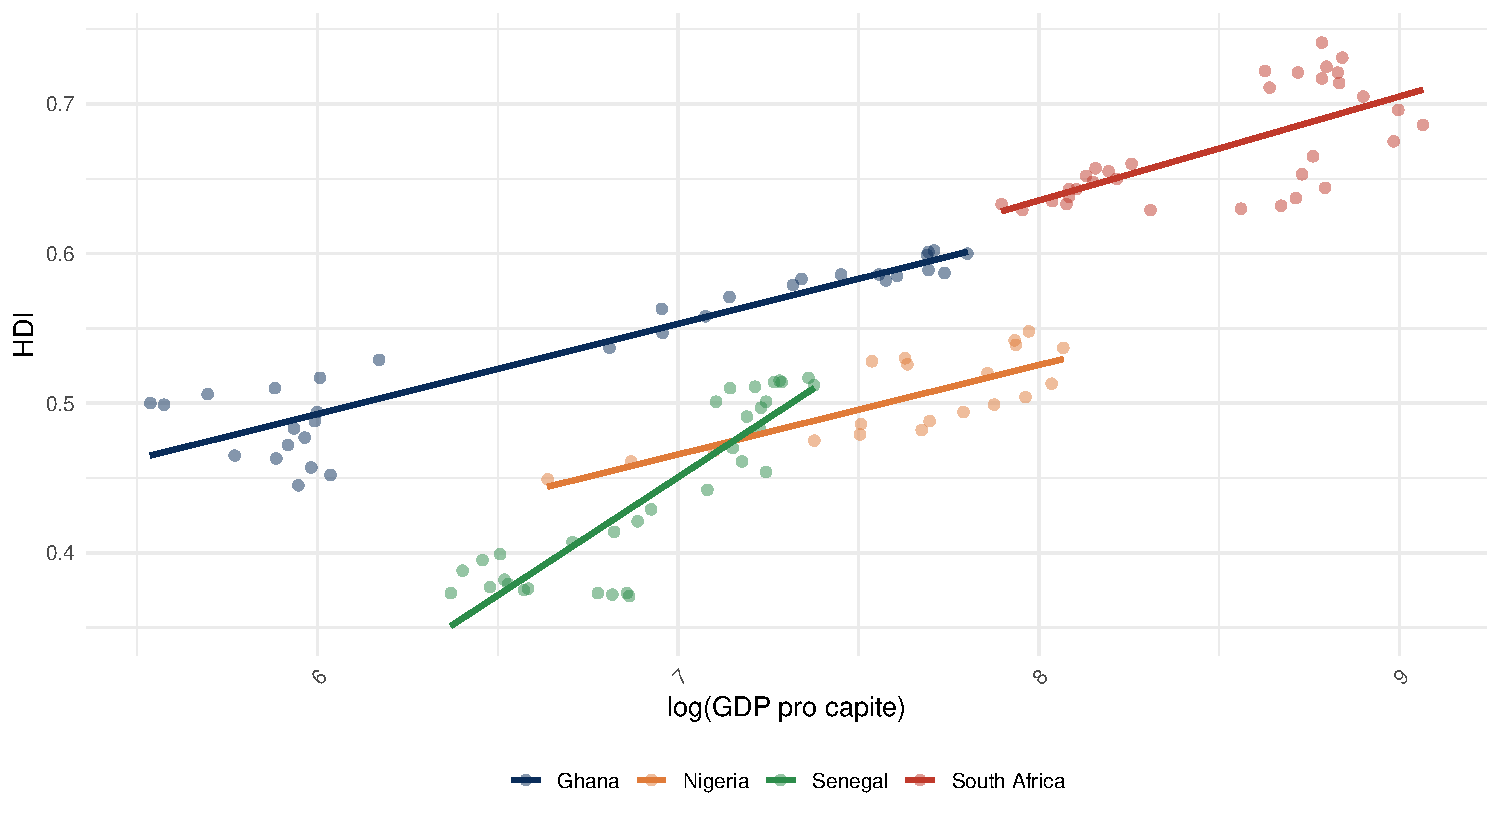
\includegraphics[width=1\linewidth,height=\textheight,keepaspectratio]{pres.final_files/figure-beamer/plot-gdp-hdi-1.pdf}

\{\footnotesize A parità di crescita del reddito, l'impatto sull'HDI
varia sensibilmente tra paesi.\}
\end{frame}

\begin{frame}{L'efficienza di trasformazione del reddito (GDP) in HDI}
\phantomsection\label{lefficienza-di-trasformazione-del-reddito-gdp-in-hdi}
\begin{itemize}
  \item \textbf{Elasticità differenziata}: I \textbf{coefficienti di interazione} rivelano che l'impatto marginale del reddito non è uniforme tra le nazioni.
  \item \textbf{Efficienza di conversione}: Un coefficiente $\log(gdp) \times \text{Paese}$ più elevato indica una maggiore capacità del sistema-paese di tradurre la crescita economica in benessere multidimensionale.
\end{itemize}

Un incremento dell'1\% del PIL pro capite produce un aumento di
\([\beta_4/100]\) punti di HDI, a parità degli altri regressori.

\begin{block}{Conclusione}
L'elasticità HDI-PIL conferma i rendimenti decrescenti della ricchezza: la crescita monetaria è condizione necessaria ma non sufficiente per il progresso umano.
\end{block}
\end{frame}

\begin{frame}{Eterogeneità tra paesi}
\phantomsection\label{eterogeneituxe0-tra-paesi}
Le interazioni misurano lo scostamento dalla categoria baseline Ghana. I
risultati non mostrano differenze significative nell'efficienza di
conversione del reddito in sviluppo umano. Tuttavia, osservando i
coefficienti di interazione, emergono pattern interessanti. Questo
suggerisce un'eterogeneità strutturale che il modello, con soli 4 paesi
e 34 anni, potrebbe non avere potenza statistica sufficiente a catturare
formalmente:

\begin{itemize}
  \item \textbf{Senegal}: tende a convertire la crescita economica in HDI più efficacemente rispetto agli altri paesi, segnalando un'architettura istituzionale più efficace nel veicolare risorse verso i pilastri dell'HDI.
  \item \textbf{Nigeria}: mostra livelli di HDI relativamente bassi rispetto al proprio PIL, suggerendo la presenza di barriere strutturali o inefficienze allocative nella spesa pubblica.
\end{itemize}
\end{frame}

\begin{frame}{Le altre variabili: Fertilità, Acqua, Elettricità e
Mortalità}
\phantomsection\label{le-altre-variabili-fertilituxe0-acqua-elettricituxe0-e-mortalituxe0}
\begin{itemize}
  \item Il \textbf{Sudafrica} registra l'HDI più alto tra i quattro paesi; la \textbf{Nigeria} il più basso — nonostante il PIL pro capite più elevato della Nigeria rispetto a Ghana e Senegal in alcuni periodi
  \item \textbf{L'impatto dei servizi di base}: L'accesso all'acqua emerge come un driver di sviluppo più robusto e immediato rispetto all'elettricità nei modelli stimati.
  \item \textbf{Fertilità}: un coefficiente negativo e significativo indica che un aumento del tasso di fertilità è associato a una diminuzione dell'HDI, probabilmente a causa dell'aumento della dipendenza demografica e della pressione sulle risorse.
\end{itemize}
\end{frame}

\begin{frame}{Modello 2 --- Aggiunta dummy di crisi}
\phantomsection\label{modello-2-aggiunta-dummy-di-crisi}
Abbiamo testato la resilienza dell'HDI agli shock globali:
\[\text{HDI}_{it} = \dots + \beta_1 D_{2008} + \beta_2 D_{2020} + \epsilon_{it}\]

\begin{itemize}
  \item Le dummy di crisi catturano shock macroeconomici esogeni (2008 e COVID-19)
  \item L’obiettivo è verificare se questi eventi hanno avuto un impatto significativo sull’HDI
  \item Le interazioni per paese permettono di valutare eterogeneità nella risposta agli shock
  \item Risultato atteso: possibile maggiore vulnerabilità nei paesi meno sviluppati
\end{itemize}
\end{frame}

\begin{frame}{Coefficienti dummy di crisi}
\phantomsection\label{coefficienti-dummy-di-crisi}
\resizebox{\textwidth}{!}{
\begin{tabular}{lrrl}
\toprule
  & Coefficiente & P-value & Sig.\\
\midrule
crisis\_2008 & 0.0028 & 0.4501 & \\
covid & 0.0056 & 0.2567 & \\
as.factor(country)Nigeria:crisis\_2008 & -0.0060 & 0.2205 & \\
as.factor(country)Senegal:crisis\_2008 & 0.0001 & 0.9841 & \\
as.factor(country)South Africa:crisis\_2008 & 0.0036 & 0.4756 & \\
\addlinespace
as.factor(country)Nigeria:covid & -0.0021 & 0.7473 & \\
as.factor(country)Senegal:covid & -0.0027 & 0.6565 & \\
as.factor(country)South Africa:covid & -0.0147 & 0.0260 & *\\
\bottomrule
\end{tabular}

}
\end{frame}

\begin{frame}{Analisi della resilienza: Shock 2008 e COVID-19}
\phantomsection\label{analisi-della-resilienza-shock-2008-e-covid-19}
\begin{itemize}
  \item \textbf{Resilienza differenziata}: I paesi con coefficienti negativi significativi per le dummy di crisi mostrano una maggiore vulnerabilità agli shock globali.
  \item \textbf{COVID-19}: Solo il Sudafrica mostra un calo significativo dell'HDI, probabilmente per la maggiore integrazione nei mercati globali (turismo, servizi)
  \item \textbf{Crisi 2008}: Nessun paese mostra un impatto statisticamente significativo. Per la Nigeria, l'effetto è negativo, suggerendo una maggiore esposizione agli shock finanziari globali.
  \item \textbf{Implicazioni politiche}: Necessità di strategie di mitigazione del rischio e diversificazione economica per aumentare la resilienza agli shock futuri, soprattutto nei paesi più vulnerabili.
\end{itemize}
\end{frame}

\begin{frame}{Sviluppi futuri e proposte di policy}
\phantomsection\label{sviluppi-futuri-e-proposte-di-policy}
\begin{block}{Riforme Istituzionali}
Per i paesi con bassa interazione, la priorità è migliorare la governance, la trasparenza e l'efficienza della spesa pubblica per tradurre meglio la crescita economica in sviluppo umano.
\end{block}

\begin{block}{Protezione sociale e prevenzione economica}
Creazione di fondi di stabilizzazione e reti di sicurezza sociale per proteggere i più vulnerabili durante shock economici, con particolare attenzione a Nigeria e Senegal.
Fondi necessari per investimenti in servizi educativi e sanitari per protezione durante le crisi future. 
\end{block}
\end{frame}

\begin{frame}{Sviluppi futuri e proposte di policy}
\phantomsection\label{sviluppi-futuri-e-proposte-di-policy-1}
\begin{block}{Diversificazione economica}
Ridurre la dipendenza da settori volatili (es. risorse naturali) e promuovere lo sviluppo di industrie manifatturiere e tecnologiche per aumentare la resil ienza economica e migliorare l'HDI a lungo termine.
\end{block}

\begin{block}{Monitoraggio e valutazione continua}
Adottare l'Elasticità sociale del reddito come nuovo KPI per valutare il successo di un goverso oltre alla crescita economica (GDP), con report annuali per monitorare i progressi verso obiettivi di sviluppo umano più inclusivi e sostenibili.
\end{block}
\end{frame}

\begin{frame}{Limiti della ricerca}
\phantomsection\label{limiti-della-ricerca}
\begin{itemize}
  \item Problemi di mancanza di dati e qualità: alcune variabili chiave (es. MPI) presentavano lacune temporali o misurazioni inconsistenti tra paesi, 
  \item Campione ridotto (4 paesi, 34 anni): potere statistico limitato per i test di diagnostica
  \item Possibile \textbf{autocorrelazione seriale} nei residui — stimatori GMM come alternativa
  \item Estendere l'analisi ad altri paesi dell'Africa Sub-Sahariana per una maggiore generalizzabilità
  \item Includere variabili istituzionali (governance, rule of law) come determinanti non economici dell'HDI
\end{itemize}

\vspace{0.5em}
\begin{center}
\textit{Grazie per l'attenzione}
\end{center}
\end{frame}




\end{document}
